\begin{figure}[htbp]
\centering
\begin{tikzpicture}
% External figure
\node[anchor=south west,inner sep=0] (image) at (0,0) {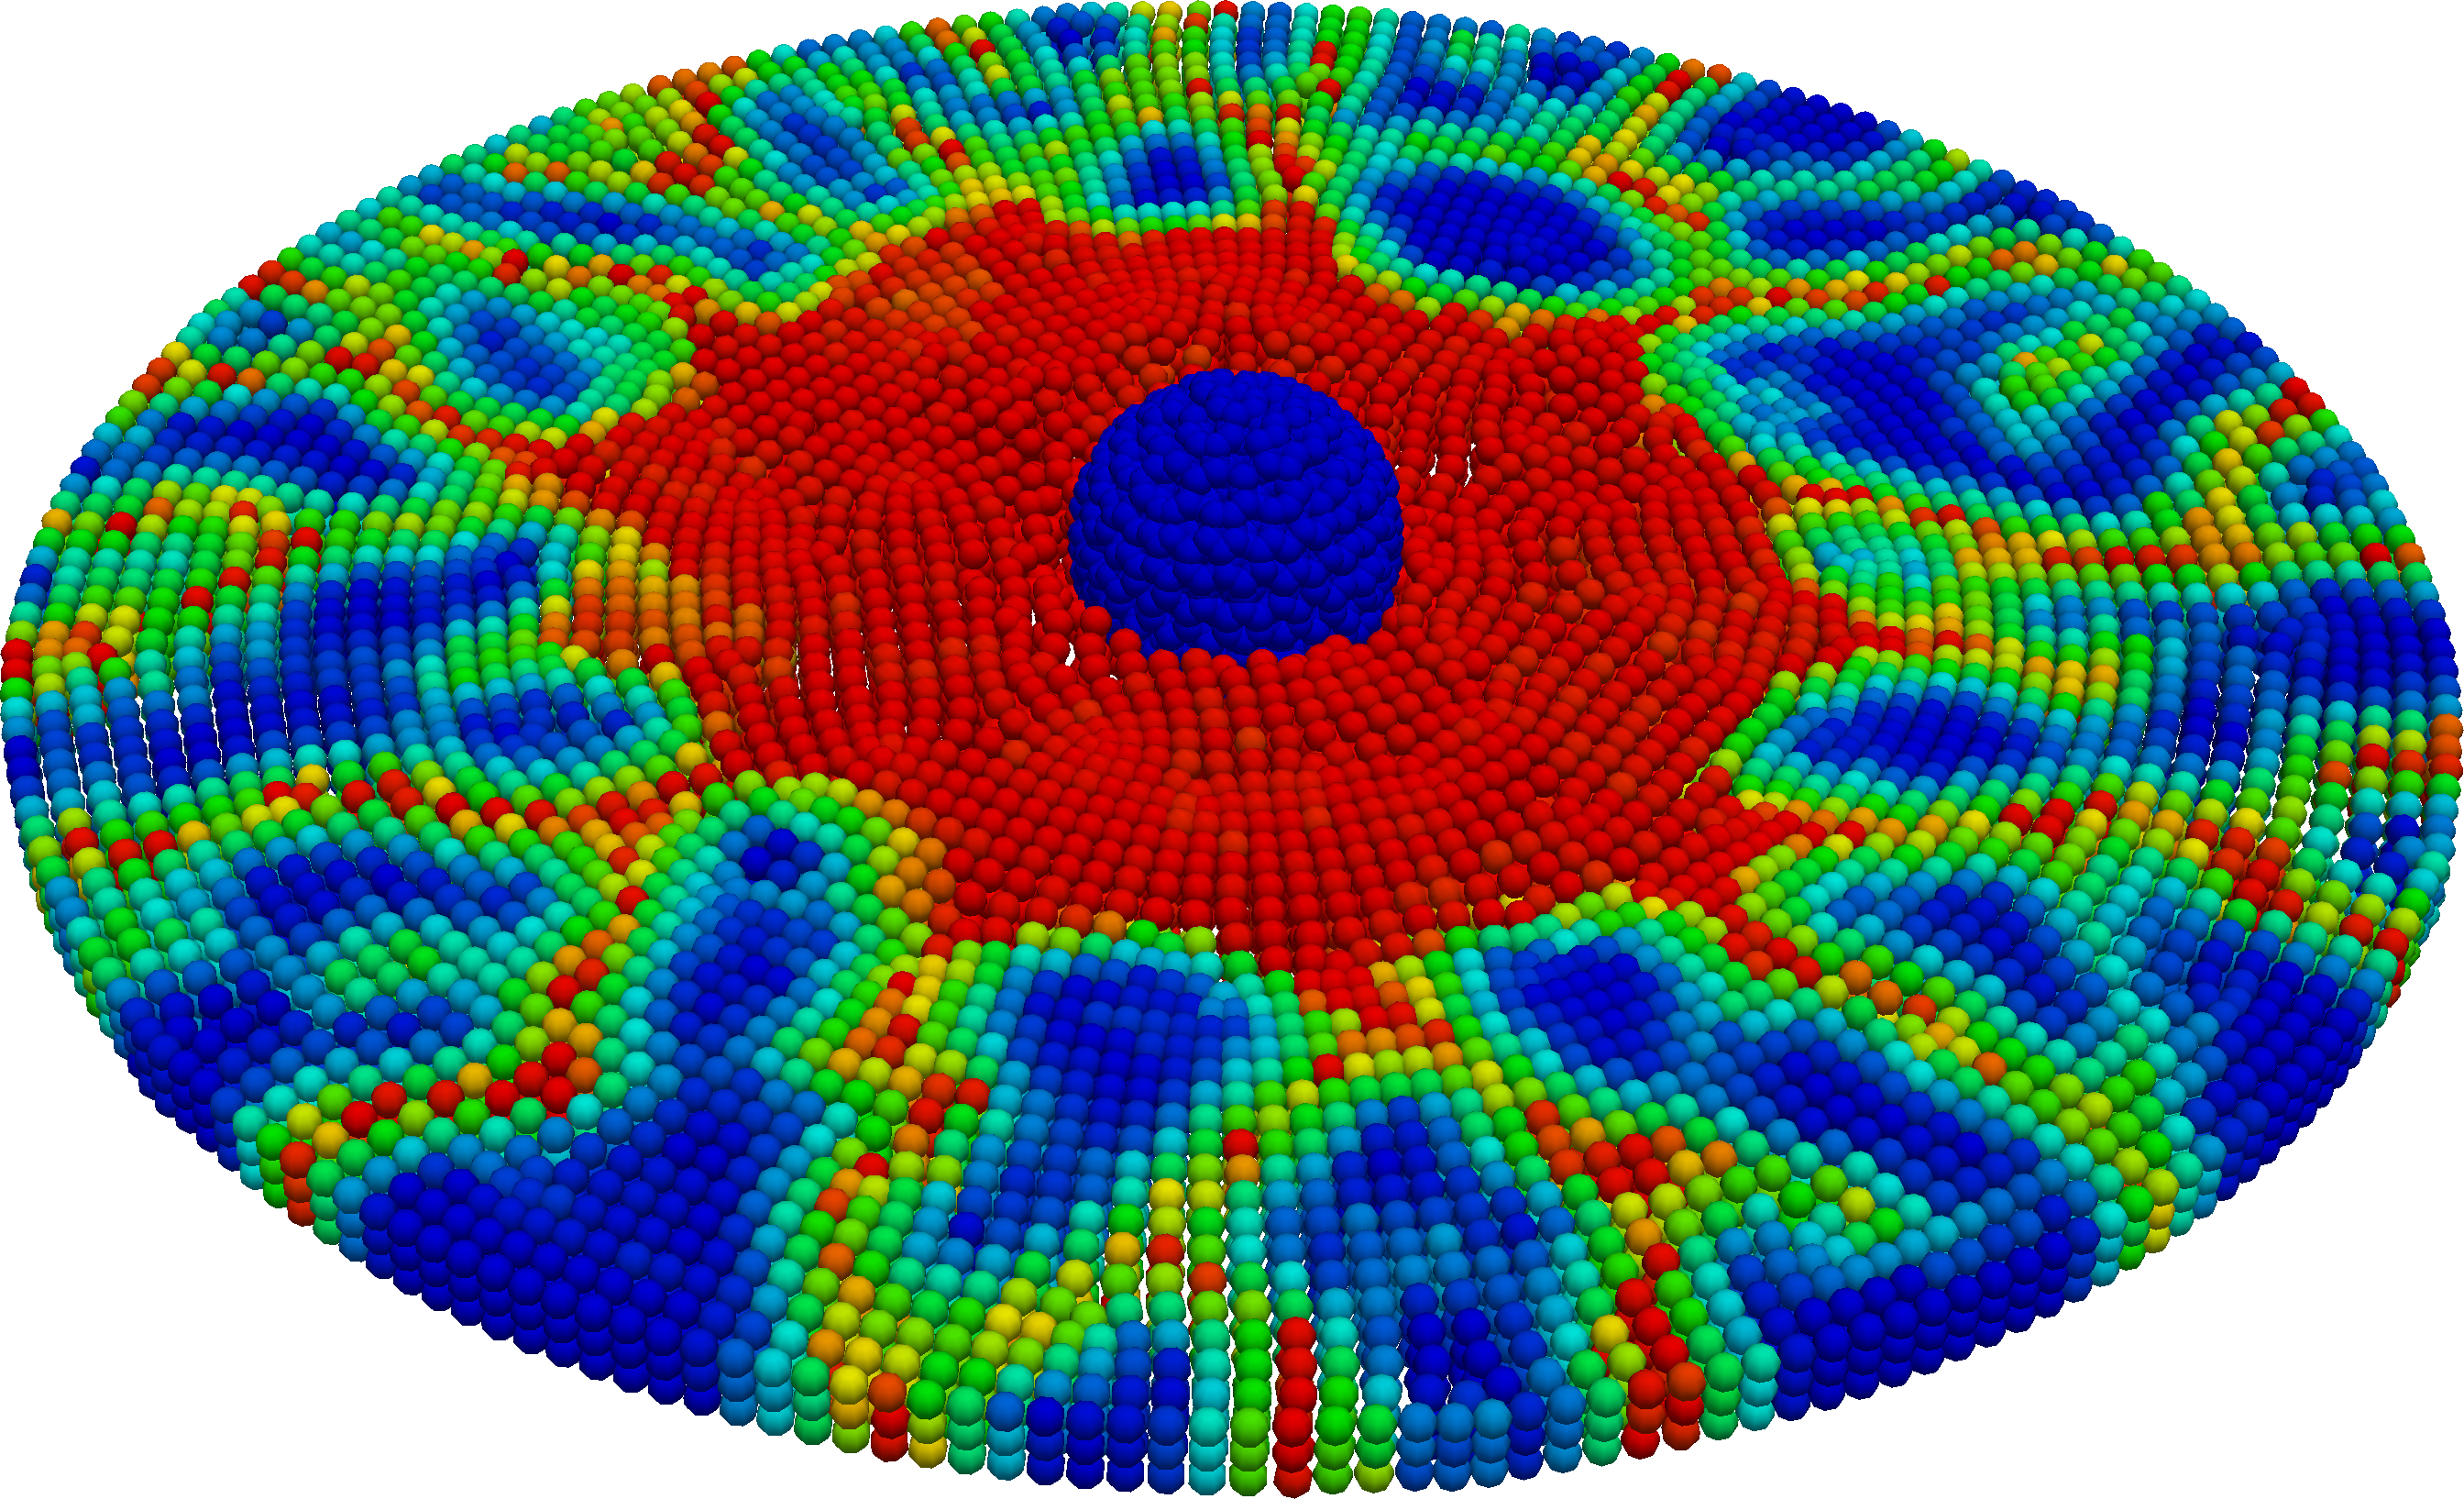
\includegraphics[width=0.7\linewidth]{Figures/Examples/Disk_Impact/Peridigm_Disk_Impact_47_Damage_ct}};
% Relative node positioning to picture
\node[anchor=east] (impactorlabel) at ($(image.west)       + (-0.5cm, 0.5)$) {Impactor};
\node[anchor=west] (disklabel)     at ($(image.south east) + ( 0.5cm,0.5)$) {Disk};
% Figure scope
\begin{scope}[
  x={(image.south east)},
  y={(image.north west)},
]
  % Some label
  \node [
    align=center,
    fill=white,
    rounded corners,
    anchor=south west
  ] at (0.05,0.1) {%
    A label with a manual linebreak\\%
    thanks to align option\\%
    using picture coordinate system%
  };
  % Some label
  \node [
    text width=3cm,
    align=center,
    fill=white,
    rounded corners
  ] at (0.75,0.65) {%
    A label with automatic linebreaks%
    thanks to text width option%
    using picture coordinate system%
  };
  % Arrows
  \draw[-latex, gray]   (impactorlabel.east) -- (0.5,0.65);
  \draw[-stealth, gray] (disklabel.west)     -- (0.9,0.2);
  % Highlight
  \draw[red,ultra thick,rounded corners] (0.72,0.05) rectangle (0.88,0.15);
  % Help grid and labels
  \draw[help lines,xstep=.1,ystep=.1] (0,0) grid (1,1);
  \foreach \x in {0,1,...,9} {\node [anchor=north] at (\x/10,0) {0.\x};}
  \foreach \y in {0,1,...,9} {\node [anchor=east]  at (0,\y/10) {0.\y};}
\end{scope}
% Outside label
\end{tikzpicture}
\caption{Labels on external picture example}
\label{fig:Labels_on_external_picture}
\end{figure}